%%% How would you use the data flow model to ensure load balancing of large scale systems?
%%% Understanding how data moves from memory, processors, and between processing nodes is
%%% essential to creating a computer architecture that avoids processor stalls common in today’s
%%% systems. The ability to map problems on to more than one processor is critical in today’s parallel
%%% processing schemes which typically struggle with cluster sizes above 16. Performers should
%%% propose (with supporting evidence) an architecture and data flow model for which memory
%%% latency, bandwidth, and capacity scale well with problem size.
\subsubsection{Power-efficient 1TB/s Link}
\label{sec:link}
\noindent
%HIVES calls for creation of processor-to-memory and processor-to-processor communication interfaces that can support extraordinarily high bandwidth exceeding 1TB/s or equivalently 8Tb/s. 
GAMA's inter-tile communication interfaces can support bandwidth exceeding 1TBps.
Providing such high bandwidth requires a total of either 800 lanes operating at 10Gb/s/lane or 320 lanes operating at 25Gb/s/lane.  
Such large number of lanes (even when spread across multiple chips) operating at high date rates poses many difficult challenges. 
For example, the total power consumption of the state-of-the-art 10mW/Gb/s links will be in excess of 80W, 
far exceeding the 20W power constraint.
%Second, interference and coupling resulting from operating a large number of closely spaced parallel lanes also severely limits performance. 
%Increasing the per lane data rate in an attempt to reduce the total number of lanes (for example, 50Gb/s/lane reduces the number of lanes to 160) is counter productive because it degrades power efficiency. 
%To elucidate this tradeoff further, increasing the data rate by a factor of 2 increases the channel loss by at least 6dB and circuit operating frequency by a factor of 2, both of which potentially increase the total by much more than 2$\times$. 
In view of this, we seek to architect new low-loss channels and connectors and improve the per lane energy efficiency to the order of 1mW/Gb/s. 
%Because the GAMA tiles are going to be designed to minimize processor idle time, dynamic power management techniques such as those described in a prior study (Anand et al., JSSC 2015) cannot be used to improve power efficiency.  Instead, the techniques that improve power efficiency at peak data are needed.


Large portion of the power consumed in multi-lane transceivers is used to perform equalization, clock generation/recovery/distribution and serializer/deserializer functions. 
We have previously developed techniques to improve power efficiency of link building blocks.
In our previous study~\cite{saxena20152}, we utilized charge-based techniques to implement equalization (both continuous-time and decision feedback), serialization and deserialization to improve link power efficiency to about 3mW/Gb/s at 14Gb/s. 
In another study~\cite{elkholy201610}, we recently demonstrated ultra low power clock generation methods using injection locking. 
At 8GHz, the prototype clock multiplier achieves about $\rm 100 fs_{rms}$-integrated jitter while consuming only 2mW, resulting in more than 5dB improvement in the jitter/power figure-of-merit. 
This low jitter makes such a clock generator suitable for 16Gb/s half-rate link architecture or even 32Gb/s quarter-rate operation. 
So far, neither circuit nor architectural techniques to lower clock distribution power have been explored. 
Further, commonly used dual-loop clock and data recovery  architecture further exacerbates this issue, as it needs multiple clocks with precise phase spacing to perform linear phase interpolation. 
In view of this, we will expand injection-locking techniques that were shown to be power and area efficient for generating low jitter clocks to also implement clock and data recovery. 
We will develop new clocking architectures that minimize clock distribution power so as to improve by the link power efficiency to 1mW/Gb/s while operating at a data rate of at least 20Gb/s.



\subsubsection{Hardware Support for Load Balancing}
\noindent
Scaling a GAMA tile to a 16-node GAMA system will face several challenges. 
First challenge is the load balancing across various  GAMA tiles. 
There are two sources of load imbalance. 
Assuming each tile may be assigned an equal number of vertices to process, but due to power law distribution some vertices may have significantly more number of edges to process. 
Fig.~\ref{fig:loadimbalance} shows a typical load balance scenario that we have noticed in our own prior work on some graph applications. 
The figure shows the wheel plots where each spoke in the wheel is the amount of computation assigned to one of 16 cores in a GPU. 
While GPU is a different baseline architecture the primary conclusion is that graph algorithms such as SSSP, BFS, APSP exhibit significant load imbalances. 
Our results also showed that this imbalance is present not only across cores but also within cores at different point in execution.  
The second source of imbalance is the barrier synchronization that may be enforced at the end of each iteration. 
For instance, well known LU decomposition algorithms iteratively compute a inverse matrix. 
While one iteration may be executed in parallel the second iteration starts only at the end of first iteration. 

 
\begin{wrapfigure}{r}[0pt]{0.4\textwidth}
\center
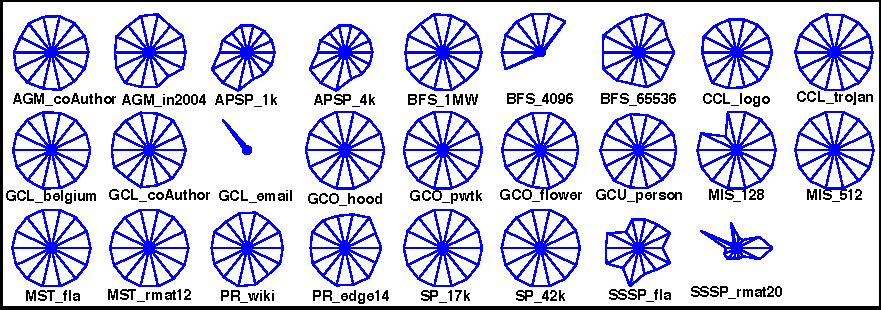
\includegraphics[width=1.0\linewidth]{./fig/load_balance_new3.pdf}
\caption{Uneven spoke lengths show computation imbalance severity}
\label{fig:loadimbalance}
\end{wrapfigure}


One way to detect the computational load is the number of NZVs that need to be processed in a row or column.  
For instance, in DCSC format it is easy to detect the number of NZVs in a column.  
The column size can be inferred from the column pointer vector.  But the number of NZVs per each column may differ significantly leading to imbalance in work. 
We plan to augment each matrix with additional metadata bits to mark the number of non-zero elements in each column in a given matrix. 
Note that these are computed during the  initial data placement in memory or when intermediate matrices are generated. These counts are only approximate since we only plan to update them infrequently. Assuming graph structure changes slowly over time we believe these approximate counters provide good first order estimate for how much computation may be assigned to a given tile or a core within a tile. We propose to assign  cores for processing vertices in proportion to the column NZV counts. However this assignment needs to be monitored at runtime due to varying memory access delays. Even if the NVZ counts are the same a given column may be laid out in memory across tiles leading to access latency imbalance. Hence, we will monitor how different tiles and cores are  progressing to identify excessive imbalances. We will rely on a simple performance counting register that counts the number of load operations completed to monitor progress. We can also use the number of elements that were fetched in to the column buffers in each GAMA core. These counters may be accessed by the  runtime or application layer to do computation migration and dynamic load balancing. 

We also propose to monitor the edge connectivity of result matrices after a computation is complete. For instance, the occurrence of a hot vertex after a graph computation step can be identified by a significant change in the sparsity corresponding to that hot vertex. Hence, we propose to provide additional monitoring registers in the GAMA tiles to measure the sparsity changes in each column. During a matrix-matrix computation, for example, we can track the change in sparsity  as the computation progresses. While maintaining this information across all vertices has high performance and memory overhead, we will only maintain this information for only a few vertices per each GAMA core as an approximation. Significant change in sparsity can be used to determine the work distribution  across GAMA tiles in the next iteration of a graph algorithm.    

With a best effort load balancing scenario we expect that some GAMA tiles will still be performing uneven amounts of work when dealing with very dynamic graphs.  We  propose to develop hardware hooks for enabling the application developer to consider relaxed synchronization approaches. When a GAMA tile is waiting at a barrier synchronization for all the tiles to finish their computation it reduces efficiency. Eliding the barrier is one approach to  improve efficiency. It has been shown in prior work that relaxed synchronization provides a tradeoff between convergence speed and resource usage efficiency and these works showed�that relaxation improves performance without impacting  convergence~\cite{bertsekas1989, baudet1978, chazan1969, uresin1989, uresin1990}.  We propose to allow the application developer to specify relaxed synchronization constraints on barrier synchronization. The programmer may specify the degree of relaxation that may be allowed across GAMA tiles before eliding the barrier. For instance, the programmer may specify elision after each GAMA tile has done at least 95\% of their computation during a iteration. The hardware then uses this information to automatically trigger a notification to software (such as through an exception) when all the GAMA tiles reach 95\% of their computation. The programmer can decide how to handle elision as part of the exception handling mechanism.  For elision, the hardware will track the progress of a given matrix operation. For a matrix-matrix multiplication operation the approximate size (number of non-zero elements) of each matrix  (stored as  metadata) is used to determine how many vertices may have been processed across all GAMA tiles periodically. That information is then gathered by a single GAMA tile that acts as a master tile, or the P8 host system to track progress. 

%For instance, one well known approach for graph clustering uses peer pressure based clustering. Every vertex votes to keep its neighbors in its own cluster and the weight of the vote is inversely proportional to edge connectivity. Based on the weighted votes the clusters are refined iteratively. But this algorithm can be represented using a matrix multiplication followed by a max computation on each iteration. The max operation waits on the parallel matrix operation to complete before computing the max. But in a relaxed synchronization approach the max computation may be initiated even before the matrix multiply operation completes. The resulting max computation may not be 

%centrality computation all pairs shortest paths may need to be computed before finding the most common vertex across all paths. Such an algorithm requires a parallel matrix-matrix multiplication

\begin{comment}


%the number of vertices in a each shortest path will determine how much computation is needed to determine the betweenness centrality in the second phase of computation. If each  

%The initial responsibility of data and computation distribution across the tiles lies with the software.  As discussed earlier, the hardware provides programming interfaces to aid the developer specify the dominant matrix access patterns. However, the hardware

%which will be used by the hardware to decide bank and channel interleaving of data. However, 
%Existing literature for parallel algorithms discusses the idea of data replication to reduce communication cost by C^1/2 or C^1/3   


%Since the GAMA system will use a distributed shared memory architecture requests that cross the tile boundaries will be 

In large-scale graph processing, communications and synchronizations amongst nodes are often the performance bottleneck.
To support efficient, scalable communications and synchronization amongst nodes, we propose two mechanisms:
(1) message passing and remote function calls; and (2) dedicated synchronization unit and relaxed synchronization.

\noindent
\textbf{Message Passing and Remote Function Calls:}
In this project communications amongst nodes, we propose a communication architecture based on message passing.

The host CPU to which the entire memory address space is visible and accessible, 
each core is restricted to access its own local memroy address space.
Thus, 
remote cores (i.e., cores in different chips).
For example, a core can remotely update a property of vertices in other remote cores by sending a message that contains the target vertex ID and the computation that will be done in the remote cores.
This is to avoid cache coherence issues among L1 data caches of cores and eliminate the need for locks to guarantee atomic updates of shared data, and facilitate the hiding of remote access latecies through asynchornous message communications.

To minimize data transfers amongst remote cores, we propose to move computations to the target remote cores that contains the data to be processed.
Building upon our proposed message passing mechanism, we propose to transfer computations as a remote function call.

\noindent
\textbf{Synchronization Unit with :} 
In many parallel graph processing frameworks, such as Bulk Synchro-nous Parallel (BSP) model, 
one of the significant bottlenecks to performance is the global synchronization that is necessary before moving across super-steps. 
We propose to design a synchronization unit whose primary responsibility is to reduce this overhead. 
As each vertex computation finishes in a super-step the sync unit tracks the progress and provides guidance for when the next super-step can begin. 
It will track inter-vertex communications to estimate which vertices are hot (namely vertices that receive most incoming messages for processing in the next super-step). 
This information can be later used to decide how to split vertices across nodes to reduce load imbalance. 
\end{comment}
